%%%%%%%%%%%%%%%%%%%%%%%%%%%%%%%%%%%%%%%%%%%%%%%%%%%%%%%%%%%%%%%%%%%%%%%
%
%  A small sample UNSW Honours Thesis file.
%  Any questions to Ian Doust i.doust@unsw.edu.au
%
% Edited CSG 11.9.2015, use some of Gery's ideas for front matter; add a conclusion chapter.
%%%%%%%%%%%%%%%%%%%%%%%%%%%%%%%%%%%%%%%%%%%%%%%%%%%%%%%%%%%%%%%%%%%%%%%
%
%  The first part pulls in a UNSW Thesis class file.  This one is
%  slightly nonstandard and has been set up to do a couple of
%  things automatically
%
 
\documentclass[honours,12pt]{unswthesis}
\linespread{1}
\usepackage{amsfonts}
\usepackage{amssymb}
\usepackage{amsthm}
\usepackage{latexsym,amsmath}
\usepackage{graphicx}
\graphicspath{{/Users/odenpetersen/Documents/Honours/order-book-hawkes/images}}
\usepackage{afterpage}
\usepackage{xcolor}

%%%%%%%%%%%%%%%%%%%%%%%%%%%%%%%%%%%%%%%%%%%%%%%%%%%%%%%%%%%%%%%%%
%
%  The following are some simple LaTeX macros to give some
%  commonly used letters in funny fonts. You may need more or less of
%  these
%
\newcommand{\R}{\mathbb{R}}
\newcommand{\Q}{\mathbb{Q}}
\newcommand{\C}{\mathbb{C}}
\newcommand{\N}{\mathbb{N}}
\newcommand{\F}{\mathbb{F}}
\newcommand{\PP}{\mathbb{P}}
\newcommand{\T}{\mathbb{T}}
\newcommand{\Z}{\mathbb{Z}}
\newcommand{\B}{\mathfrak{B}}
\newcommand{\BB}{\mathcal{B}}
\newcommand{\M}{\mathfrak{M}}
\newcommand{\X}{\mathfrak{X}}
\newcommand{\Y}{\mathfrak{Y}}
\newcommand{\CC}{\mathcal{C}}
\newcommand{\E}{\mathbb{E}}
\newcommand{\cP}{\mathcal{P}}
\newcommand{\cS}{\mathcal{S}}
\newcommand{\A}{\mathcal{A}}
\newcommand{\ZZ}{\mathcal{Z}}
%%%%%%%%%%%%%%%%%%%%%%%%%%%%%%%%%%%%%%%%%%%%%%%%%%%%%%%%%%%%%%%%%%%%%
%
% The following are much more esoteric commands that I have left in
% so that this file still processes. Use or delete as you see fit
%
\newcommand{\bv}[1]{\mbox{BV($#1$)}}
\newcommand{\comb}[2]{\left(\!\!\!\begin{array}{c}#1\\#2\end{array}\!\!\!\right)
}
\newcommand{\Lat}{{\rm Lat}}
\newcommand{\var}{\mathop{\rm var}}
\newcommand{\Pt}{{\mathcal P}}
\def\tr(#1){{\rm trace}(#1)}
\def\Exp(#1){{\mathbb E}(#1)}
\def\Exps(#1){{\mathbb E}\sparen(#1)}
\newcommand{\floor}[1]{\left\lfloor #1 \right\rfloor}
\newcommand{\ceil}[1]{\left\lceil #1 \right\rceil}
\newcommand{\hatt}[1]{\widehat #1}
\newcommand{\modeq}[3]{#1 \equiv #2 \,(\text{mod}\, #3)}
\newcommand{\rmod}{\,\mathrm{mod}\,}
\newcommand{\p}{\hphantom{+}}
\newcommand{\vect}[1]{\mbox{\boldmath $ #1 $}}
\newcommand{\reff}[2]{\ref{#1}.\ref{#2}}
\newcommand{\psum}[2]{\sum_{#1}^{#2}\!\!\!'\,\,}
\newcommand{\bin}[2]{\left( \begin{array}{@{}c@{}}
				#1 \\ #2
			\end{array}\right)	}
%
%  Macros - some of these are in plain TeX (gasp!)
%
\newcommand{\be}{($\beta$)}
\newcommand{\eqp}{\mathrel{{=}_p}}
\newcommand{\ltp}{\mathrel{{\prec}_p}}
\newcommand{\lep}{\mathrel{{\preceq}_p}}
\def\brack#1{\left \{ #1 \right \}}
\def\bul{$\bullet$\ }
\def\cl{{\rm cl}}
\let\del=\partial
\def\enditem{\par\smallskip\noindent}
\def\implies{\Rightarrow}
\def\inpr#1,#2{\t \hbox{\langle #1 , #2 \rangle} \t}
\def\ip<#1,#2>{\langle #1,#2 \rangle}
\def\lp{\ell^p}
\def\maxb#1{\max \brack{#1}}
\def\minb#1{\min \brack{#1}}
\def\mod#1{\left \vert #1 \right \vert}
\def\norm#1{\left \Vert #1 \right \Vert}
\def\paren(#1){\left( #1 \right)}
\def\qed{\hfill \hbox{$\Box$} \smallskip}
\def\sbrack#1{\Bigl \{ #1 \Bigr \} }
\def\ssbrack#1{ \{ #1 \} }
\def\smod#1{\Bigl \vert #1 \Bigr \vert}
\def\smmod#1{\bigl \vert #1 \bigr \vert}
\def\ssmod#1{\vert #1 \vert}
\def\sspmod#1{\vert\, #1 \, \vert}
\def\snorm#1{\Bigl \Vert #1 \Bigr \Vert}
\def\ssnorm#1{\Vert #1 \Vert}
\def\sparen(#1){\Bigl ( #1 \Bigr )}

\newcommand\blankpage{%
    \null
    \thispagestyle{empty}%
    \addtocounter{page}{-1}%
    \newpage}

%%%%%%%%%%%%%%%%%%%%%%%%%%%%%%%%%%%%%%%%%%%%%%%%%%%%%%%%%%%%%%
%
% These environments allow you to get nice numbered headings
%  for your Theorems, Definitions etc.  
%
%  Environments
%
%%%%%%%%%%%%%%%%%%%%%%%%%%%%%%%

\newtheorem{theorem}{Theorem}[section]
\newtheorem{lemma}[theorem]{Lemma}
\newtheorem{proposition}[theorem]{Proposition}
\newtheorem{corollary}[theorem]{Corollary}
\newtheorem{conjecture}[theorem]{Conjecture}
\newtheorem{definition}[theorem]{Definition}
\newtheorem{example}[theorem]{Example}
\newtheorem{remark}[theorem]{Remark}
\newtheorem{question}[theorem]{Question}
\newtheorem{notation}[theorem]{Notation}
\numberwithin{equation}{section}

%%%%%%%%%%%%%%%%%%%%%%%%%%%%%%%%%%%%%%%%%%%%%%%%%%%%%%%%%%%%%%%%%%
%
%  If you've got some funny special words that LaTeX might not
% hyphenate properly, you can give it a helping hand:
%
\hyphenation{Mar-cin-kie-wicz Rade-macher}

%%%%%%%%%%%%%%%%%%%%%%%%%%%%%%%%%%%%%%%%%%%%%%%%%%%%%%%%%%%%%%%%%%
% 
% OK...Now we get to some actual input.  The first part sets up
% the title etc that will appear on the front page
%
%%%%%%%%%%%%%%%%%%%%%%%%%%%%%%%%%%%%%%%%%%%%%%%%%%%%%%%%%%%%%%%%%

\title{Point Process Modelling of a Limit Order Book}

\authornameonly{Oden Petersen}

\author{\Authornameonly\\{\bigskip}Supervisor: Dr. Tom Stindl}

\copyrightfalse
\figurespagefalse
\tablespagefalse

%%%%%%%%%%%%%%%%%%%%%%%%%%%%%%%%%%%%%%%%%%%%%%%%%%%%%%%%%%%%%%%%%
%
%  And now the document begins
%  The \beforepreface and \afterpreface commands puts the
%  contents page etc in
%
%%%%%%%%%%%%%%%%%%%%%%%%%%%%%%%%%%%%%%%%%%%%%%%%%%%%%%%%%%%%%%%%%%

\begin{document}

\beforepreface

\afterpage{\blankpage}

% plagiarism

\prefacesection{Plagiarism statement}

\vskip 10pc \noindent I declare that this thesis is my
own work, except where acknowledged, and has not been submitted for
academic credit elsewhere. 

\vskip 2pc  \noindent I acknowledge that the assessor of this
thesis may, for the purpose of assessing it:
\begin{itemize}
\item Reproduce it and provide a copy to another member of the University; and/or,
\item Communicate a copy of it to a plagiarism checking service (which may then retain a copy of it on its database for the purpose of future plagiarism checking).
\end{itemize}

\vskip 2pc \noindent I certify that I have read and understood the University Rules in
respect of Student Academic Misconduct, and am aware of any potential plagiarism penalties which may 
apply.\vspace{24pt}

\vskip 2pc \noindent By signing 
this declaration I am
agreeing to the statements and conditions above.
\vskip 2pc \noindent
Signed: \rule{7cm}{0.25pt} \hfill Date: \rule{4cm}{0.25pt} \newline
\vskip 1pc

\afterpage{\blankpage}

% Acknowledgements are optional


\prefacesection{Acknowledgements}

\afterpage{\blankpage}

% Abstract

\prefacesection{Abstract}

This is the abstract
\afterpage{\blankpage}


\afterpreface

\afterpage{\blankpage}

\chapter{Introduction}\label{s-intro}

{\noindent}Modern financial markets facilitate the exchange of shares and other financial assets at extremely high frequency. The ability to trade throughout the day allows market participants to respond to exogenous news and endogenous market events in a manner that minimises their risk and generates profits over the long term. Intraday trading activity has a significant influence on the formation of market pricesm and plays a key role in reducing transaction costs while increasing the speed at which large institutions can control their exposure to various financial risks and opportunities.

Securities exchanges play a key role in this ecosystem, facilitating the automated matching of buyers and sellers at prices favourable to both. Understanding the dynamics of this exchange process at a high degree of resolution can provide insights into the design of automated \textit{matching engines} that produce desirable market behaviour, as well as insights into the design of \textit{trading strategies} that exploit the dynamics of the exchange process to generate profits.

\section{Limit Order Books}
A matching engine is tasked with receiving and acting on various messages from market participants indicating their intent to buy or sell a particular security with particular conditions. As a result of this process, trades may be formed that match buyers and sellers at a mutually agreeable price and quantity. Trade reports are broadcast to relevant participants and may be used for the purposes of risk management and forecasting, as well as for the ultimate transfer of the assets that have been traded (which often occurs after trading hours).

\bigskip

A typical matching engine permits two kinds of incoming messages, known as \textit{order insertion} and \textit{order cancellation}, and maintains an internal state consisting of a single data structure, known as a \textit{limit order book}.

\medskip

An order insertion message indicates a participant's willingness to buy (or sell) some quantity of a particular asset at or below (respectively, above) a particular price, and results in the addition of an \textit{order} to the limit order book.

Conversely, an order cancellation message results in the removal of a particular order from the limit order book. \textcolor{red}{It might be good to include a statistic about roughly how large cancellation rates are, to highlight the importance of this message type.}

Formally, a limit order book can be defined as a set of tuples (``orders'') of the form
$$(\text{side},\text{price},\text{time},\text{size})\in \{-1,1\}\times P\times T\times Q,$$
where
\begin{itemize}
	\item The order expresses an intention to buy (side$=1$) or sell (side$=-1$) the asset
	\item The price of the order is a real number. Typically prices are restricted to some discrete set of values, and the difference between successive prices is known as the \textit{tick size} (usually constant).
\end{itemize}


\textcolor{red}{I plan to also highlight in this section some key features of limit order book structures, such as the definition of bid/ask levels, the mechanics of the matching process and queue priority, and the evolution of the limit order book over time, motivating the emphasis on modeling arrival times. I also plan to highlight the fact that queue depletions are intimately related to price changes; this is discussed in the Bouchaud source and seems like important motivation.}

\section{Point Process Models of Book Updates}
With the goal of modelling the arrival time process, we now turn to an introductory overview of point processes, and highlight some key variants described in existing literature that are relevant to this application.

\textcolor{red}{
For each extension:
- show some example realisations for various parameter choices: barcode and intensity plot
}

\subsection{Point Processes}

%For each of these variations, maybe use a common example throughout (e.g. arrival times of trades) for clarity.

Given a sample space $\Omega$ with probability measure $\mathbb P$, a point process is any increasing random sequence of times $$\mathcal T:\Omega\to{\mathbb{R}_{\geq 0}}^\mathbb{N}.$$
These times are often referred to as \textit{event times}, with the implication that the sequence represents the times at which some event of interest occurs (for instance, the arrival of messages sent to a matching engine).

{\noindent}For any point process, there exists a corresponding nondecreasing random function $N_{\mathcal T}:\mathbb{R}_{\geq 0}\times\Omega\to\mathbb{N}$ known as the \textit{counting process}, that gives the number of times having occurred before or at a given time. This is defined as
$$N_{\mathcal T}(t,\omega) = \vert \{i\in\mathbb N \vert \mathcal{T}(\omega)_i \leq t\} \vert.$$

{\noindent}All \textcolor{red}{(or perhaps many)} of the point processes considered in this thesis will additionally be \textit{adapted point processes}, in the sense that $N_{\mathcal T}$ is a stochastic process adapted with respect to some filtration $\mathcal F$.

\textcolor{red}{Perhaps I should define here what a filtration is?}

{\noindent}A point process $\mathcal T$ may also be \textit{marked}, in which case it is associated with one or more random sequences of marks $\mathcal E:\Omega\to E^{\mathbb N}$ drawn from a set $E$, typically representing additional information about each event. A common special case of this is when $E$ is finite, in which case we may refer to the elements of $E$ as \textit{event types}, and refer to $\mathcal T$ as a \textit{multivariate point process} with a \textit{multivariate counting process}
$${\tilde N}_{\mathcal T, \mathcal E} : \mathbb{R}_{\geq 0}\times\omega \to \mathbb N ^ {\vert E \vert}$$
$$N_{\mathcal T, \mathcal E}(t,\omega)_e = \vert \{i\in\mathbb N \vert \mathcal{T}(\omega)_i \leq t, \mathcal{E}(\omega)_i=e\} \vert.$$

\subsection{The Expectation Measure}
Let $B(\mathbb{R})$ be the Borel $\sigma$-algebra on $\mathbb R$.
\textcolor{red}{Does the $\sigma$-algebra need to be this restricted, or can it just be $\mathcal{P}(\mathbb{R})$?}

{\noindent}For any point process $\mathcal T$ and for any $\omega\in\Omega$, we can define the \textit{counting measure} $\Lambda_\omega$ as
$$\Lambda_\omega : B(\mathbb R) \to \mathbb{N}$$
$$\Lambda_\omega(S) = \left\vert S\cap \mathcal{T}(\omega)\right\vert.$$

Taking the expectation of the counting measure with respect to $\mathbb{P}$ (optionally conditional on some sub-$\sigma$-algebra of $\Omega$) gives the \textit{expectation measure} $\Lambda(S)$.

\textcolor{red}{For the sake of intuition, it should probably be shown here that $d\Lambda=d(\mathbb{E}N)$}

\textcolor{red}{It is also important to define the expectation measure with respect to a sigma-algebra, and in particular one from the filtration.}

\subsection{Intensity Functions}
\textcolor{red}{These can be formulated using the Radon-Nikodym derivative of $\Lambda$ with respect to the lebesgue measure on time, i.e. $d\Lambda=\lambda dt$.}
\textcolor{red}{For intuition, this is the arrival rate.}

\subsection{Poisson Processes}
Probably the simplest modeling assumption we can make is to assume that the arrival rate of the process is a constant \textcolor{red}{conditional on any sigma-algebra in the filtration to which the process is adapted}.

A Poisson process is a point process for which the following two properties hold.
\begin{enumerate}
	\item For any collection of disjoint Borel sets $B\subset B(\mathbb R)$, their couting measures $\{\Lambda_w(b) : b\in B\}$ are independent random variables.
	\item For any Borel set $b$ with finite Lebesgue measure $\mu(b)$, we have $\Lambda(b)=\lambda \mu(b)\propto \mu(b)$ for some fixed $\lambda\in\mathbb{R}$. \textcolor{red}{Put differently, we have $d\Lambda=\lambda dt$.}
\end{enumerate}

\textcolor{red}{This definition might require a reference.}

\textcolor{red}{Multivariate case}

\textcolor{red}{There is a link here to the sante fe order book model, described in the Bouchaud source, which is an example of the application of poisson arrivals.}

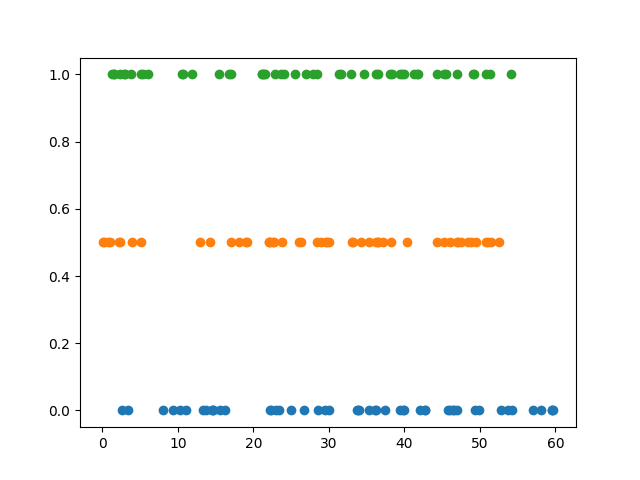
\includegraphics[width=0.75\textwidth]{poisson_sim.png}

\textcolor{red}{I think I should change this to be separate plots. Can show the intensity function for each; e.g. for inhomogenous it's the same for every realisation, but for hawkes process the intensity function is itself random.}


\subsection{Inhomogeneous Poisson Process}
An inhomogeneous Poisson process is a generalisation of the Poisson process for which the second condition is replaced by the weaker requirement that every Borel set $b$ with finite Lebesgue measure $\mu(b)$ has a finite expectation measure. \textcolor{red}{Is this weaker version even needed, or is it sufficient to just drop the condition entirely?}

\subsection{Autoregressive Intensity \& Hawkes Processes}
\textcolor{red}{Intuitively, self-excitation or self-inhibition}

immigration/birth interpretation

\subsection{State-dependent Hawkes Processes}
Moriaru-Patrichi and Pakkanen find that conditioning on the state of the order book improves the fit of the model.

They consider conditioning on only the state of the triggering event (their 2.3), as well as conditioning on both the state of the triggering event and the current state (their 4.2).

The first of these:
	$$\tilde\lambda_{ex}(t)=\phi_e(X(t),x)\left(\nu_e+\sum_{e'\in\mathcal E,x'\in \mathcal X}\int_{[0,t)}k_{e',e}(t-s,x')d\tilde N_{e'x'}(s)\right), & t\geq 0, & e\in\mathcal E, & x\in\mathcal X.$$

The second:
	$$\tilde\lambda_{ex}(t)=\nu_{ex}+\sum_{e'\in\mathcal E,x'\in\mathcal X}\int_{[0,t)}k_{e'x'ex}(t-s)d\tilde N_{e'x'}(s), t\geq 0, e\in\mathcal E, x\in\mathcal X.$$

\chapter{Estimation}

\section{Introduction to estimation algorithms}
\subsection{MLE}
\subsection{EM}
\subsection{Bayesian Approach}
- Uncertainty quantification
- Less likely to get stuck in local optima

\section{Prior work on estimation}

\chapter{Application to NYSE Data}

%{\noindent}Given a sequence $\{x_n\}_{n=1}^{\infty}$ in a Banach space $\X$,
%the following natural questions may be asked.  %\begin{enumerate} %\item[(Q1)] Which elements of the space $\X$ can be expressed in the form %$\sum_{n=1}^{\infty}a_nx_n$ for some unique sequence $\{a_n\}_{n=1}^{\infty}$
%of scalars?
%
%\item[(Q2)] Supposing $x\in\X$ can be written as $\sum_{n=1}^{\infty}a_nx_n$,
%does it matter in what order the terms of the series are summed?
%
%\item[(Q3)] In the setting of (Q2), will the series
%$\sum_{n=1}^{\infty}\varepsilon_na_nx_n$ converge for any choice of
%$\varepsilon_n=\pm 1$?
%
%\item[(Q4)] Given a scalar sequence $\{\phi_n\}_{n=1}^{\infty}$, does it give
%rise to a bounded linear mapping
%$\sum_{n=1}^{\infty}a_nx_n\mapsto\sum_{n=1}^{\infty}\phi_na_nx_n$?
%\end{enumerate}
%
%{\noindent}Answering these and similar questions for
%function spaces whose members act on the circle group $\T\cong[0,2\pi]$
%is the main subject of this thesis.
%
%In Chapter 1, we give a general picture of the situation, introducing the
%concepts of Schauder bases and conditional convergence of sequences in Banach
%spaces. Standard examples show that not every Banach space with a basis
%$\{x_n\}_{n=1}^{\infty}$ has the property that the terms in each expansion 
%$\sum_{n=1}^{\infty}a_nx_n$ can be freely rearranged.
%
%
%The above questions have been the subject of much study for the trigonometric
%sequence $\{x_n\}_{n=-\infty}^{\infty}$ contained in $\X=L^p(\T)$ and given by
%$x_n(t)=e^{int}$. If $1<p<\infty$, then it is known that
%$\{x_n\}_{n=-\infty}^{\infty}$ is a basis for $\X$. Moreover, each $f\in\X$ has
%the expansion
%\begin{equation}\label{intro1}
%f=\sum_{n=-\infty}^{\infty}a_nx_n
%\end{equation}
%where the series converges in $\X$ and for each $n\in\Z$,
%\begin{equation}\label{intro2}
%a_n=\frac{1}{2\pi}\int_0^{2\pi}e^{-ins}f(s)\,ds.
%\end{equation}
%In Chapter 2 we give an account of this theory in as much as it applies to
%answering questions similar to those above. In particular, we recall three
%classical results from harmonic analysis --- the M. Riesz Conjugacy Theorem,
%the Littlewood--Paley Theorem and the Strong Marcinkiewicz Multiplier Theorem.
%These demonstrate that the expansion (\ref{intro1}) is valid for each 
%$f\in L^p(\T)$ (for $1<p<\infty$) and give sequences
%$\{\phi_n\}_{n=1}^{\infty}$ for which (Q4) has a positive answer.
%
%In Chapter 3 we present some results of Bourgain
%which generalise these classical theorems to the $L^p(\T,\Y)$ spaces
%--- those $L^p$ spaces whose functions take values in a Banach space $\Y$. 
%When
%$\Y$ is a Banach space that has the so-called UMD property and when 
%$1<p<\infty$,
%analogues of the M. Riesz, Littlewood--Paley and Marcinkiewicz Theorems hold. In
%particular, equation (\ref{intro1}) is valid if $f$ belongs to any of these
%function spaces.
%
%After examining these vector-valued function spaces, we look at functions on
%$\T$ which are operator-valued. A certain class of functions, whose members are
%strongly continuous group homorphisms of $\T$ into $\B(\Y)$, yields analogues of
%the M. Riesz, Littlewood--Paley and Marcinkiewicz Theorems if
%$\Y$ has the UMD property.
%These analogues were first announced in the 1980s and 1990s by Berkson
%and Gillespie (see \cite{BG Fourier} and \cite{BG Spectral}). They are stated
%in Chapter 4, where it is also shown how they
%specialise to the classical theorems. In particular, given a strongly continuous
%representation $R:\T\rightarrow\B(\Y)$, its `Fourier series'
%\[R=\sum_{n=-\infty}^{\infty}P_nx_n,\]
%converges. The $n$th `Fourier coefficient' $P_n$ of $R$ is a projection
%on $\Y$ given by the formula
%\[P_n=\frac{1}{2\pi}\int_0^{2\pi}e^{ins}R(s)\,ds.\]
%The similarity between the above two equations and equations (\ref{intro1}) and
%(\ref{intro2}) is striking.
%
%Proving the theorems stated in Chapter 4 is the main objective of 
%Chapters 5 and 6. Contained in the proofs are a wide range of techniques
%taken from harmonic analysis and Banach space operator theory. 
%The parts of the proofs of the two main theorems are dispersed across the 
%literature with significant portions being found in
%\cite{BBG}, \cite{BG Fourier}, \cite{BG Spectral}, \cite{BGM} and \cite{Bourg}.
%These chapters provide what is most likely the only unified account of these
%proofs. Chapter 6 ends
%with an example that demonstrates the scope of these theorems. Applying the
%Strong Marcinkiewicz analogue for strongly continuous representations, a wide
%class of multiplier
%projections acting on the von Neumann Schatten $\CC_p$ spaces are given. This
%class was recently discovered by Doust and Gillespie (see \cite{DG}).
%
%This thesis is a coherent presentation of a quest to generalise three classical
%theorems that were discovered in the 1920s, 1930s and 1940s. Their analogues are
%the product of a conglomeration of ideas that straddle the 1980s and 1990s and
%the application of these new results brings the story into the twenty-first
%century.
%
%
%
%%%%%%%%%%%%%%%%%%%%%%%%%%%%%%%%%%%%%%
%
%\chapter{Convergence and Bases on Banach Spaces}
%
%%%%%%%%%%%%%%%%%%%%%%%%%%%%%%%%%%%%%%
%
%
%In this chapter we outline the general context in which our study of multiplier
%theory in Banach spaces
%takes place. We begin by revising the elementary concepts
%associated with functional analysis in Banach spaces. Then Section \ref{bases}
%introduces the notions of bases, multiplier transforms and unconditional
%convergence of sequences, setting the scene for the rest of the thesis. The 
%chapter ends by introducing a technique which is frequently used to obtain 
%results pertaining to the unconditionality of sequences.
%
%
%%%%%%%%%%%%
%\section{Banach, Operator and Dual Spaces}\label{Banach Spaces}
%%%%%%%%%%%%
%
%We recall some basic definitions and concepts from Banach space theory and
%functional analysis. A good introductory reference for this material is 
%\cite{Con}.
%
%A {\em Banach space} $\X$ is a vector space $V$ over a field $\F$ that is 
%equipped with a norm
%$\norm{\,\cdot\,}_{\X}$ that makes $V$ complete with respect to the metric $d$
%given by $d(x,x')=\norm{x-x'}_{\X}$. In this thesis we shall always assume that
%the
%underlying field $\F$ of scalars is $\C$. Suppose $\Y$ is also a Banach space
%with norm $\norm{\,\cdot\,}_{\Y}$. A linear operator
%$T:\X\rightarrow\Y$ is said to be {\em bounded} if
%$\sup\{\norm{Tx}_{\Y}:x\in\X,\norm{x}_{\X}=1\}<\infty$. The collection of
%$\Y$-valued bounded linear operators on $\X$ is denoted $\B(\X,\Y)$, and is
%itself a Banach space when equipped with the {\em operator norm}
%$\norm{T}=\sup\{\norm{Tx}_{\Y}:x\in\X,\norm{x}_{\X}\leq 1\}$. A $\Y$-valued
%linear
%operator on $\X$ is bounded if and only if it is continuous with respect to the
%topologies on $\X$ and $\Y$ induced by their respective norms. Furthermore, if
%$T\in\B(\X,\Y)$ then $\norm{Tx}_{\Y}\leq\norm{T}\norm{x}_{\X}$ for all $x\in\X$.
%
%Henceforth, the norm of a Banach space $\X$ will be denoted
%$\norm{\,\cdot\,}_{\X}$ (except when $\X$ is an $L^p$ space --- see the
%example below), while the operator norm $\norm{\,\cdot\,}$ will
%contain no subscript because it is clear from the operator's definition what
%spaces its norm is induced from. The space $\B(\X,\X)$ of bounded linear
%operators sending elements of $\X$ into $\X$ will be denoted $\B(\X)$. An
%important class of operators included in $\B(\X)$ are the {\em projections} on
%$\X$, those bounded linear maps $P$ satisfying $P^2=P$.
%
%There are many examples of Banach spaces. We give one example that will feature
%regularly throughout the thesis.
%
%\begin{example}\label{L^p example}
%Let $(\Omega,\A,\mu)$ be a measure space and $1\leq p<\infty$. Let
%$\X=L^p(\Omega,\A,\mu)$ be the space of all equivalence classes of
%$\C$-valued $\A$-measurable functions $f$ on $\Omega$ with the property that
%$\int_{\Omega}|f(x)|^p\,d\mu(x)<\infty$. We shall usually blur the distinction
%between the equivalence classes of $L^p(\Omega,\A,\mu)$ and the representatives
%of these classes. The norm on $\X$ is given by
%$\norm{f}_{\X}=(\int_{\Omega}|f(x)|^p\,d\mu(x))^{1/p}$ and
%makes $\X$ a Banach space. When the underlying $\sigma$-algebra and measure is
%standard (for example, when $\Omega=\R$, $\A$ is the Borel $\sigma$-algebra
%and $\mu$ is Lebesgue measure on $\R$), we shall denote
%$L^p(\Omega,\A,\mu)$ by $L^p(\Omega)$. 
%Because it
%is notationally less cumbersome to write $\norm{\,\cdot\,}_p$ instead of
%$\norm{\,\cdot\,}_{L^p(\Omega,\A,\mu)}$, we shall do so whenever the context
%permits no ambiguity. A particularly useful fact is that if $(\Omega,\A,\mu)$ is
%a finite measure space and $1\leq p<r<q\leq\infty$, then
%$L^p(\Omega)\cap L^q(\Omega)\subset L^r(\Omega)$ and
%$L^q(\Omega)\subset L^p(\Omega)$. A quick source of information on these spaces
%is \cite[\S 6.4]{Pedersen}.
%\end{example}
%
%\begin{example}
%We give a few of the sequence spaces. 
%\begin{enumerate}
%\item For $1\leq p<\infty$, define $\lp$ to be
%the space of all functions $f:\N\rightarrow\C$ such that
%$\sum_{n=1}^{\infty}|f(n)|^p<\infty$, and equip it with the norm
%$\norm{f}_{\lp}=(\,\sum_{n=1}^{\infty}|f(n)|^p\,)^{1/p}$. Thus $\lp$ may be
%identified with $L^p(\N)$, where the underlying measure is counting measure on
%$\N$.
%\item The space $\ell^{\infty}$ is the set of all bounded functions
%$f:\N\rightarrow\C$ with norm $\norm{f}_{\ell^{\infty}}=\sup\{|f(n)|:n\in\N\}$.
%\item The subset $c$ of $\ell^{\infty}$ of all convergent sequences 
%has norm given by $\norm{f}_c=\norm{f}_{\ell^{\infty}}$ for $f\in c$.
%\item The subset $c_0$ of $\ell^{\infty}$ of all bounded functions converging to
%zero has norm given by $\norm{f}_{c_0}=\norm{f}_{\ell^{\infty}}$ for $f\in c_0$.
%\end{enumerate}These are all Banach spaces.
%\end{example}
%
%To every Banach space is associated another Banach space known as its dual.
%Suppose $\X$ is a Banach space. A {\em linear functional} on $\X$ is a linear
%map from $\X$ into $\C$. The set of all bounded linear functionals on $\X$,
%denoted
%by $\X^*$, is made a vector space via pointwise operations. We equip $\X^*$ with
%a norm given by $\norm{x^*}_{\X^*}=\sup\{|x^*(x)|:x\in\X,\norm{x}\leq 1\}$.
%Thus $\X^*$ coincides with $\B(\X,\C)$ and is itself a Banach
%space. We call $\X^*$ the {\em dual space} of $\X$. Given $x^*\in\X^*$ and
%$x\in\X$, it is standard to write
%$\ip<x,x^*>$ for $x^*(x)$.
%
%It can be shown that for $1<p<\infty$, the dual space of $\X=L^p(\Omega,\A,\mu)$
%is isometrically isomorphic to $\X=L^q(X,\Omega,\mu)$, where $q$ satisfies
%$1/p+1/q=1$. Thus $(\lp)^*$ is isomorphic to $\ell^q$ as a Banach space. It is
%also known that $c_0^*=\ell^1$ and $(\ell^1)^*=\ell^{\infty}$. See
%\cite[Chapter III, \S 5 and \S 11]{Con} for more details.
%
%Given a Banach space $\X$, we may take its dual $\X^*$. This is also a Banach
%space and hence has a dual $(\X^*)^*$, called {\em the second dual of $\X$}
%and written $\X^{**}$. Continuing in this way we may construct a sequence
%$\X,\X^*,\X^{**},\X^{***},\ldots$ of Banach spaces. For which
%spaces $\X$ does this list contain any repetitions? This question leads us to
%consider an important class of Banach spaces, known as the reflexive Banach
%spaces.
%
%Let $\X$ be Banach space. To each $x\in\X$ we may associate a unique element
%$\hatt{x}\in\X^{**}$ by the rule $\hatt{x}(x^*)=\ip<x,x^*>$ for all $x^*\in\X$.
%The map $x\mapsto\hatt{x}$ from $\X$ into $\X^{**}$ is called the {\em natural
%map} of $\X$ into its second dual.
%
%A Banach space $\X$ is said to be {\em reflexive} if
%$\X^{**}=\{\hatt{x}:x\in\X\}$. If $\X$ is reflexive then its second dual
%$\X^{**}$ is isometrically isomorphic to $\X$. However, the converse does not
%hold (see \cite[III.11]{Con}). It is a consequence of the Riesz Representation
%Theorem \cite[I.3.4]{Con} that every Hilbert space is reflexive.
%The spaces $\X=L^p(X,\Omega,\mu)$ and
%$\lp$ are also reflexive for $1<p<\infty$, but by the above remarks $c_0$ is 
%not. Since
%$c_0^{**}=\ell^{\infty}$, it is clear that $c_0\subset c_0^{**}$. In fact,
%$c_0$ is isometrically embedded into its second dual $\ell^{\infty}$. This fact
%generalises to
%all Banach spaces. The space $C[0,1]$ of continuous functions on $[0,1]$ with
%supremum norm is another example of a non-reflexive Banach space.
%
%A {\em Banach algebra} $\mathfrak{A}$ is an algebra over $\F$ that has a norm
%$\norm{\,\cdot\,}_{\mathfrak{A}}$ relative to which $\mathfrak{A}$ is a Banach
%space and
%\[\norm{ab}_{\mathfrak{A}}\leq\norm{a}_{\mathfrak{A}}\norm{b}_{\mathfrak{A}}\]
%for all $a,b\in\mathfrak{A}$. If $\mathfrak{A}$ has an identity $e$, then it is
%assumed that $\norm{e}_{\mathfrak{A}}=1$. In this thesis we shall always take
%$\F$ to be $\C$. An example of a Banach algebra is the space $C[0,1]$ equipped
%with the supremum norm, with multiplication of elements in $C[0,1]$ defined
%pointwise.
%
%
%%%%%%%%%%%%%
%\section{Topologies in Banach Spaces}\label{topologies}
%%%%%%%%%%%%%
%
%A Banach space $\X$ is easily made a topological space with the topology induced
%by its norm, called the {\em norm topology} of $\X$. We say a sequence of
%vectors {\em converges in $\X$} if it converges in the norm topology of $\X$.
%Another
%topology is the {\em weak topology} of $\X$. A sequence $\{x_n\}_{n=1}^{\infty}$
%of vectors in $\X$ converges to $x\in\X$ in the weak topology of $\X$ if
%$\lim_{n\rightarrow\infty}\ip<x_n-x,x^*>=0$ for all $x^*\in\X^*$. As their names
%suggest, convergence in the norm topology implies convergence in the weak
%topology, or in other words, if a sequence converges then it also converges
%weakly.
%
%We shall consider three topologies in the Banach space $\B(\X)$.
%Suppose $\{T_n\}_{n=1}^{\infty}$ is a sequence of operators in $\B(\X)$.
%We say it
%converges to $T$ {\em in norm} if $\norm{T-T_n}\rightarrow 0$, {\em strongly} if
%$\norm{Tx-T_nx}_{\X}\rightarrow 0$ for all $x\in\X$, and {\em weakly} if
%$\ip<Tx-T_nx,x^*>\rightarrow 0$ for all $x\in\X$ and $x^*\in\X^*$. The 
%topologies
%induced are called the norm operator topology, the strong operator topology and
%the weak
%operator topology of $\B(\X)$ respectively. A sequence which converges strongly
%will converge weakly, and in turn, convergence in the norm topology implies
%strong convergence. All three topologies have unique limits and distinguish
%points.
%
%The following proposition is easy to verify and is included for familiarisation
%with the concepts discussed thus far. It shall also be used to establish later
%results.
%
%\begin{proposition}\label{SOT convergence}
%Let $\X$ be a Banach space and suppose $\{T_n\}_{n=1}^{\infty}$ is a sequence of
%operators uniformly bounded in norm by some $K>0$ and converging to $T$
%in the strong operator topology of $\B(\X)$. Then $\norm{T}\leq
%K$.
%\end{proposition}
%
%\begin{proof}
%We want to show $\norm{Tx}_{\X}\leq K\norm{x}_{\X}$ for all $x\in\X$. Fix
%$x\in\X$ and $\epsilon>0$ and choose an $n\in\N$ such that
%$\norm{Tx-T_nx}_{\X}<\epsilon$. Then 
%\[\norm{Tx}_{\X}\leq\norm{Tx-T_nx}_{\X}+\norm{T_nx}_{\X}
%<\epsilon+K\norm{x}_{\X},\]
%and the proposition follows.
%\end{proof}
%
%
%
%%%%%%%%%%%%%
%\section{Bases in Banach spaces}\label{bases}
%%%%%%%%%%%%%
%
%
%The definition and usefulness of a basis in a finite dimensional vector space is
%well-known. It is natural then to want an analogous concept for
%Banach spaces. The most useful approach is found in the notion of a Schauder
%basis. A comprehensive introduction to such bases is \cite[pp. 1--52]{Lind},
%upon which most of the material in this section is based. 
%
%\begin{definition}
%A sequence $\{x_n\}_{n=1}^{\infty}$ in a Banach space $\X$ is called a {\em 
%Schauder basis of $\X$} if, for every $x\in\X$, there is a unique sequence of
%scalars $\{a_n\}_{n=1}^{\infty}$ such that $x=\sum_{n=1}^{\infty}a_nx_n$. A
%sequence $\{x_n\}_{n=1}^{\infty}$ which is a Schauder basis for its closed
%linear span is called a {\em basic sequence}.
%\end{definition}
%
%A Banach space $\X$ is called {\em separable} if it has a countable dense 
%subset.
%Thus if $\X$ has a Schauder basis then $\X$ is separable. In general the 
%converse
%is not true. Since the class of Schauder bases is the only type of bases
%considered in this
%thesis, it will henceforth be implicit that any discussion about bases refers
%only to Schauder bases.
%
%
%\begin{example}
%The ordered set of unit vectors $e_n=(0,0,0,\ldots,1,0,\ldots)$, where the $1$
%occurs in the $n$th coordinate, forms a basis in each of the spaces
%$c$, $c_0$ and $\lp$. Another example of a basis in $c$ is given by
%$x_1=(1,1,1,\ldots)$
%and $x_n=e_{n-1}$ for $n>1$. If $x=(b_1,b_2,\ldots)\in c$, then the expansion of
%$x$ with respect to this basis is
%\[x=(\lim_{k\rightarrow\infty}a_k)x_1+(a_1-\lim_{k\rightarrow\infty}a_k)x_2+
%(a_2-\lim_{k\rightarrow\infty}a_k)x_3+\cdots.\] 
%\end{example}
%
%
%If a Banach space $\X$ has a basis, we may consider $\X$ as a sequence
%space via an identification of each element $x=\sum_{n=1}^{\infty}a_nx_n$ in
%$\X$ with the unique sequence of coefficients $(a_1,a_2,a_3,\ldots)$. To do this
%note that it is essential to describe the basis as an ordered sequence rather
%than merely as a set. The following example highlights a deeper reason for
%why we must specify the ordering of the vectors in a basis.
%
%\begin{example}\label{summing basis}
%Consider the sequence of vectors $\{x_n\}_{n=1}^{\infty}$ in $c$ given by
%\[x_n=(\underbrace{0,0,\ldots,0}_{n-1},1,1,\cdots),\]
%for $n\in\Z^+$. It is not hard to see that this is a basis for $c$.
%It is called the {\em summing basis} in $c$.
%Consider the sequence $b$ defined by
%\[b_n=\sum_{k=1}^n(-1)^{k+1}\frac{1}{k}\]
%for $n\in\Z^+$. By Leibniz' test for alternating series,
%$b_n$ has a limit as $n\rightarrow\infty$, so $b\in c$. The expansion of $b$ 
%with
%respect to the summing basis is $b=\sum_{n=1}^{\infty}a_nx_n$ where
%$a_n=(-1)^{n+1}\frac{1}{n}$. Now consider the following rearrangement of the
%series. Define $\pi:\Z^+\rightarrow\Z^+$ by
%\[\pi(n)=\left\{\begin{array}{ll}
%				2k & \mbox{if $n=3k$}\\
%				4k+1 & \mbox{if $n=3k+1$}\\
%				4k+3 & \mbox{if $n=3k+2$.}
%			\end{array}\right.
%\]
%Then $\pi$ is clearly a permutation of $\Z^+$. However, the expansion
%\[b'\equiv\sum_{n=1}^{\infty}a_{\pi(n)}x_{\pi(n)}\]
%does not lie in $c$ since
%\[b_{3n}'=\sum_{k=1}^n\left(\frac{1}{2k-1}+\frac{1}{2k+1}-\frac{1}{2k}\right)
%\geq 2\sum_{k=1}^n\frac{1}{k}\]
%diverges as $n\rightarrow\infty$.
%\end{example}
%
%Not every basis has the defect that the convergence of an expansion with respect
%to the basis is dependent on the order of summation of the expansion. For
%example, expansions in finite dimensional spaces can be summed in any order
%without altering convergence. The following proposition gives various methods 
%for
%checking whether a sum of vectors can be freely rearranged while still
%respecting convergence.
%
%\begin{proposition}\label{unconditional conv}
%\cite[Proposition 1.c.1]{Lind}
%Let $\{x_n\}_{n=1}^{\infty}$ be a sequence of vectors in a Banach space $\X$.
%Then the following are equivalent.
%
%(i) The series $\sum_{n=1}^{\infty}x_{\pi(n)}$ converges for every permutation
%$\pi$ of the integers.
%
%(ii) The series $\sum_{k=1}^{\infty}x_{n_k}$ converges for every choice of
%$n_1<n_2<n_3\ldots$.
%
%(iii) The series $\sum_{n=1}^{\infty}\varepsilon_nx_n$ converges
%for every choice of signs $\varepsilon_n=\pm 1$.
%
%(iv) For every $\epsilon>0$ there exists an integer $n_0$ such that
%$\ssnorm{\sum_{j\in J}x_j}_{\X}<\epsilon$ for every finite set of integers $J$
%which satisfies $\min\{j\in J\}>n_0$.
%\end{proposition}
%
%With the aid of the proposition, there are now easier ways to verify that the
%series
%$\sum_{n=1}^{\infty}a_nx_n$ given in Example \reff{bases}{summing basis} is
%dependent on the order of summation. Simply observe that
%$\sum_{n=1}^{\infty}a_{2n-1}x_{2n-1}$ does not converge in $c$ and hence 
%statement (ii) of the proposition fails to hold.
%
%\begin{definition}
%Let $\{x_n\}_{n=1}^{\infty}$ be a sequence of vectors in a Banach space $\X$.
%A series $\sum_{n=1}^{\infty}x_n$ which satisfies any of the conditions (i),
%(ii), (iii) or (iv) in Proposition \reff{bases}{unconditional conv} is said to 
%be
%{\em unconditionally convergent}. A basis $\{x_n\}_{n=1}^{\infty}$ of a Banach
%space $\X$ is {\em unconditional} if for every $x\in\X$, its expansion
%$x=\sum_{n=1}^{\infty}a_nx_n$ converges unconditionally. Otherwise the basis is
%said to be {\em conditional}.
%\end{definition}
%
%Thus the standard ordered bases $\{e_n\}_{n=1}^{\infty}$ for $c$, $c_0$ and
%$\lp$,
%$1\leq p<\infty$ are unconditional bases. This means that any reordering of
%$\{e_n\}_{n=1}^{\infty}$ also yields unconditional bases in these spaces.
%The summing basis for $c$ is clearly a conditional basis.
%
%Given a basis $\{x_n\}_{n=1}^{\infty}$, one might ask what
%complex sequences $\{\phi_n\}_{n=1}^{\infty}$ give rise to a bounded multiplier
%transform? That is, is there a constant $C>0$ such that for all $x\in\X$,
%\[\snorm{\sum_{n=1}^{\infty}\phi_na_{n,x}x_n}_{\X}\leq C\norm{x}_{\X},\]
%where $\sum_{n=1}^{\infty}a_{n,x}x_n$ is the expansion of each $x\in\X$ with
%respect to the basis? If that basis is unconditional, then the space of such
%sequences is just $\ell^{\infty}$ (see \cite[Proposition 1.c.7]{Lind}).
%
%
%We have seen that conditional bases do exist, and some of the resulting
%difficulties that arise when working with a conditional basis. Is there any way
%in which we can avoid such problems in separable Banach spaces? In other words,
%can we always find an unconditional
%basis for a separable Banach space? The answer is no. The space $L^1[0,1]$ has
%no unconditional basis. In fact, $L^1[0,1]$ cannot even be embedded in a space
%with an unconditional basis \cite[Propostion 1.d.1]{Lind}.
%
%There are many open problems regarding unconditional bases. For example,
%suppose $\X$ is a Banach space with an unconditional basis, and let $\Y$ be
%a complemented subspace of $\X$. Does $\Y$ have an unconditional basis? One
%outstanding problem has recently been solved (see \cite{Gowers}).
%Does every infinite dimensional Banach space $\X$ contain an unconditional
%basic sequence? The answer is no.
%We shall not pursue such broad problems in this thesis. Instead, we shall use 
%tools from harmonic analysis and spectral theory to examine whether or not
%particular sequences in certain Banach spaces are conditional, and whether or 
%not
%they form bases for those spaces.
%
%
%
%
%
%%%%%%%%%%%%%%%%%%%%%%%%%%%%%%%%%%%%%%%%%%%%%%%%%%%%%%%%%%%%%%%%%%%%%
%
%\chapter{Classical Harmonic Analysis}\label{cha}
%
%%%%%%%%%%%%%%%%%%%%%%%%%%%%%%%%%%%%%%%%%%%%%%%%%%%%%%%%%%%%%%%%%%%%%
%
%
%
%
%We now
%leave the broad discussion about bases and conditionality in Banach spaces and
%instead focus our attention to some particular classes of the $L^p$ Banach
%spaces. The theory of classical harmonic analysis provides a good starting point
%from which to tackle problems relating to bases and conditionality in this 
%setting.
%
%In this chapter we give an overview of some basic results from classical
%harmonic analysis and Fourier theory.
%We begin by introducing the fundamental concepts of harmonic analysis on locally
%compact Abelian groups. The Fourier transform and Fourier multipliers will be
%defined. Connections between multiplier transforms and convolution operators 
%will
%be drawn in Section \ref{lca}, as well as important examples given. In
%Section \ref{lca} we discuss some of the classical results of M. Riesz,
%Littlewood--Paley and Marcinkiewicz.
%
%The general theory given in this chapter can be used to consider the
%the set of functions $\{\varphi_n\}_{n\in\Z}\subset L^p(\T)$, where
%$\varphi_n:t\mapsto e^{int}$. Is this a basis for the Banach space $L^p(\T)$?
%Is it an unconditional basic sequence? If not, how close is it
%to being an unconditional sequence? The results stated in Section 
%\ref{lca}
%answer such questions.
%
%
%
%
%%%%%%%%%%%%%%%%%
%\section{Harmonic Analysis on Locally Compact Abelian Groups}\label{lca}
%%%%%%%%%%%%%%%%%
%
%
%In this section we give the necessary background from which we can begin to
%answer
%the questions from
%above. The theory mentioned here can be found in \cite{Katznelson}
%and is quite 
%standard. In what follows, if $G$ is a group, the inverse of an
%element $x\in G$ will be denoted by $-x$, and the group operation from
%$G\times G$ into $G$ will be denoted by $(x,y)\mapsto x+y$. 
%
%
%\begin{definition} A {\em locally compact Abelian group} (or an LCA group)
%$G$ is an Abelian group
%which is also a locally compact Hausdorff space such that the group operations
%$x\mapsto -x$ from $G$ onto $G$ and $(x,y)\mapsto x+y$ from $G\times G$
%onto $G$ are continuous. 
%\end{definition}
%
%The most-studied examples of LCA groups are the integers $\Z$, the circle group
%$\T$ and real line $\R$ with their usual topologies. 
%It is easy to verify that any Abelian group can be made into an LCA group
%when endowed with the discrete topology. In this thesis the circle group $\T$
%will feature most often. It can be modelled by the unit circle
%$\{\omega\in\C:|\omega|=1\}$
%in the complex plane, or as the quotient group $\R/2\pi\Z$. We shall usually
%adopt the latter model,
%thinking of $\T$ as the interval $[0,2\pi]$ with endpoints identified and
%addition as the group operation.
%
%A good reason to study LCA groups is
%that we can use them to construct measure spaces that are translation invariant.
%
%\begin{definition} Let $G$ be a locally compact Abelian group. A {\em Haar
%measure} on $G$ is a positive regular Borel measure $\mu$ having the
%following two properties:
%
%(i) $\mu(E)<\infty$ if $E\subseteq G$ is compact; and
%
%(ii) $\mu(E+x)=\mu(E)$ for all measurable $E\subseteq G$ and all $x\in G$.
%\end{definition}
%
%\begin{theorem}\cite[Chapter VII, \S 2]{Katznelson}
%Let $G$ be an LCA group. Then a Haar measure on $G$ exists and is unique up to
%multiplication of a positive constant.
%\end{theorem}
%
%Hence one often speaks of {\em the} Haar measure. For $G=\T$, Haar measure is
%usually taken to be normalised
%Lebesgue measure, $(2\pi)^{-1}dt$. If $G$ is discrete and infinite, Haar measure
%is usually
%normalised to have mass one at each point. We denote the $L^p$ space of
%functions on $G$ with respect to Haar measure by $L^p(G)$. As mentioned in
%Example \reff{Banach Spaces}{L^p example}, we will not usually distinguish
%between functions defined on $G$ and their $L^p$ equivalence classes.
%
%Using Haar measure, we may turn $L^1(G)$ into a Banach algebra.
%
%\begin{theorem}\label{convolution}
%Let $G$ be an LCA group with Haar measure $dy$
%and suppose $f,g\in L^1(G)$. Then for almost all $x\in G$, the function
%$y\mapsto f(x-y)g(y)$ for $y\in G$ is integrable on $G$.
%If we write 
%\[h(x)=\int_G f(x-y)g(y)dy,\]
%then $h\in L^1(G)$ and $\norm{h}_1\leq\norm{f}_1\norm{g}_1$.
%\end{theorem}
%
%\begin{definition} Let $G,f,g$ be as in Theorem \reff{lca}{convolution}. Then
%the {\em convolution} of $f$ and $g$, denoted $f*g$, is given by
%\[(f*g)(x)=\int_G f(x-y)g(y)dy\]
%for almost all $x\in G$
%\end{definition}
%
%\begin{corollary} Let $G$ be an LCA group. Then $L^1(G)$ is a
%Banach Algebra under convolution and pointwise addition.
%\end{corollary}
%
%Our next aim is to define the Fourier transform of a function in $L^1(G)$.
%We start by introducing the characters of $G$.
%
%\begin{definition} A {\em character} on an LCA group $G$ is a continuous mapping
%$\xi$ from $G$ into $\C$ such that $|\xi(x)|=1$
%and $\xi(x+y)=\xi(x)\xi(y)$ for all $x,y\in G$. The set of all characters of
%$G$ is denoted $\hatt{G}$.
%\end{definition}
%
%Thus a character is a continuous homomorphism of $G$ into $\T$. It can be shown
%that the set of characters on $\T$ is the set $\{\varphi_n\}_{n\in\Z}$, where
%$\varphi_n(t)=e^{int}$ for all $n\in\Z$ and all $t\in[0,2\pi]$. Every character
%of
%$\Z$ has the form $n\mapsto e^{int}$ for some $t\in[0,2\pi]$. The characters of
%$\R$ are all of the form $x\mapsto e^{ixy}$ for some $y\in\R$.
%
%For any LCA group $G$, the set of characters $\hatt{G}$ can be made 
%an Abelian group. We shall denote its group operation by $+$ (in what follows, 
%this should cause no confusion with the group operation $+$ for $G$) and
%define it by $(\xi_1+\xi_2)(x)=\xi_1(x)\xi_2(x)$ for all $x\in G$.
%We write $\ip<x,\xi>$ for $\xi(x)$.
%
%A topology is defined on $\hatt{G}$ by specifying that
%$\{\xi_n\}_{n=1}^{\infty}\subset\hatt{G}$ converges to $\xi\in\hatt{G}$ if
%$\{\xi_n\}_{n=1}^{\infty}\subset\hatt{G}$ converges uniformly to $\xi$ on all
%compact subsets of $G$. It can be shown that this topology turns $\hatt{G}$ into
%a locally compact Abelian group (see \cite[Chapter VII, \S 3]{Katznelson}).
%We say that $\hatt{G}$ is the {\em dual group}
%of $G$.
%
%The {\em Pontryagin Duality Theorem} (see \cite[p.189]{Katznelson}) asserts
%that, for $x\in G$
%and $\xi\in\hatt{G}$, the mapping $\xi\mapsto \ip<x,\xi>$ is a character on
%$\hatt{G}$, and every character on $\hatt{G}$ is of this form. Moreover, the
%topology induced by uniform convergence on compact subsets of $\hatt{G}$
%coincides with the original topology on $G$. In otherwords, if $\hatt{G}$ is the
%dual group of $G$, then $G$ is the dual of $\hatt{G}$.
%
%We illustrate the Pontryagin Duality Theorem for the LCA group $\T$.
%We saw that there exists a
%bijection between $\hatt{\T}$ and $\Z$, since given any $\xi\in\hatt{\T}$, there
%is a unique $n\in\Z$ such that $\ip<t,\xi>=e^{int}$ for all $t\in\T$.
%Moreover, the topology $\hatt{T}$ is the
%discrete topology. Thus $\hatt{\T}\simeq\Z$. One may similarly show that
%$\hatt{\Z}\simeq\T$. This duality may be described (by abuse of notation) as
%$\ip<n,t>=e^{int}=\ip<t,n>$ for
%all $t\in\T$ and all $n\in\Z$. (On
%the left hand side, we regard $n$ as an element of $\Z$ while on the right
%hand side we regard it as a function on $\T$.)
%
%We now have all the tools needed to define the Fourier transform of an 
%integrable
%function on an LCA group.
%
%\begin{definition}\label{Fourier transf}
%Let $G$ be an LCA group. Then the {\em
%Fourier transform} of a function $f\in L^1(G)$ is defined by
%\[\hatt{f}(\xi) = \int_G \overline{\ip<y,\xi>}f(y)dy\]
%for all $\xi\in\hatt{G}$, where $dy$ is Haar measure on $G$.
%\end{definition}
%
%Thus the Fourier transform of a function $f\in L^1(\Z)$ is
%\[\hatt{f}(t)=\sum_{n=-\infty}^{\infty}e^{-int}f(n)\]
%for all $t\in\T$, since Haar measure on $\Z$ is unit point-mass measure.
%Similarly, the Fourier transform of a function $f\in L^1(\T)$ is
%\[\hatt{f}(n) = \frac{1}{2\pi}\int_0^{2\pi}e^{-int}f(t)dt\]
%for all $n\in\Z$, where $dt$ is Lebesgue measure. The {\em Fourier series} of
%$f$ is the corresponding formal expression
%\[\sum_{n=-\infty}^{\infty}\hatt{f}(n)\varphi_n\]
%where $\varphi_n(t)=e^{int}$ for all $t\in\T$ and all $n\in\Z$.
%
%
%We aim to use the Fourier transform to construct a large class of operators
%which act on the $L^p$ space of a given LCA group. We may do this via {\em
%Plancherel's Theorem}.
%
%\begin{theorem}\label{isometry}\cite[Chapter VII, \S 4]{Katznelson}
%{\em Plancherel's Theorem.} Let $G$ be a locally compact Abelian group. Then the
%Fourier transform on $L^1(G)$ is an isometry of $L^1\cap L^2(G)$ onto a dense
%subspace of $L^2(\hatt{G})$. Hence it can be extended to an isometry of $L^2(G)$
%onto $L^2(\hatt{G})$.
%\end{theorem}
%
%For the circle group $\T$, Plancherel's theorem takes the following form.
%
%\begin{theorem}\label{Plancherel for T}\cite[Theorem I.5.5]{Katznelson}
%
%(i) Let $f\in L^2(\T)$. Then
%\[\sum_{n=\infty}^{\infty}|\hatt{f}(n)|^2=
%\frac{1}{2\pi}\int_0^{2\pi}|f(t)|^2\,dt,\]
%that is, $\ssnorm{\hatt{f}}_{L^2(\Z)}=\norm{f}_{L^2(\T)}$.
%
%(ii) For each $f\in L^2(\T)$,
%\[f=\lim_{N\rightarrow\infty}\sum_{n=-N}^N\hatt{f}_n\varphi_n\]
%in $L^2(\T)$ norm, where $\varphi_n:t\mapsto e^{int}$.
%
%(iii) Given any sequence $\{a_n\}_{n=-\infty}^{\infty}$ of complex numbers in
%$L^2(\Z)$, then there exists a unique $f\in L^2(\T)$ such that
%$a_n=\hatt{f}(n)$.
%
%Thus the correspondence $f\leftrightarrow\{\hatt{f}(n)\}_{n=-\infty}^{\infty}$
%is an isometry between $L^2(\T)$ and $L^2(\Z)$.
%\end{theorem}
%
%
%A by-product of the above theorem is that the set $\{\varphi_n\}_{n\in\Z}$ of
%functions in the Hilbert space $L^2(\T)$ forms a complete orthonormal system 
%(and
%hence an unconditional basis) with respect to the inner product
%\[\ip<f,g>=\frac{1}{2\pi}\int_0^{2\pi}f(t)\overline{g(t)}\,dt.\]
%
%It is harder to establish whether or not $\{\varphi_n\}_{n\in\Z}$ is a basis for
%$L^p(\T)$ when $1\leq p<\infty$ and $p\neq2$. Standard results about Fej\'{e}r's
%kernel (see Section \ref{lca} and \cite[I.2.6]{Katznelson}) give the following
%facts. First recall that a {\em trigonometric polynomial} is a function on 
%$\T$ of 
%the form $\sum_{n=-N}^Na_n\varphi_n$ where $N\in\N$ and $a_n\in\C$.
%
%\begin{theorem}\label{Fejer facts}
%Fix $1\leq p<\infty$. Then
%
%(i) the trigonometric polynomials are dense in $L^p(\T)$;
%
%(ii) if $f,g\in L^p(\T)$ and $\hatt{f}(n)=\hatt{g}(n)$ for all $n\in\Z$,
%then $f=g$; and
%
%
%(iii) if the Fourier series of a function $f\in L^p(\T)$ does converge in
%$L^p$-norm, then it converges to $f$.
%\end{theorem}
%
%So if the Fourier series does converge for each function in $L^p(\T)$,
%$\{\varphi_n\}_{n\in\Z}$ is a basis for $L^p(\T)$. Otherwise,
%one would like to know whether or not $\{\varphi_n\}_{n\in\Z}$ is a basic 
%sequence in $L^p(\T)$ for $p\neq2$, and whether this sequence is unconditional.
%One way to study such problems is through multiplier transforms.
%
%\begin{definition}\label{multipliers}
%Let $G$ be an LCA group and let
%$\phi:\hatt{G}\rightarrow\C$ be bounded and measurable on $\hatt{G}$. By
%Plancherel's Theorem, define $S_{\phi}$ to be the continuous linear mapping of
%$L^2(G)$ into itself for which
%$({S_{\phi}f})\,\hatt{\,} = \phi \hatt{f}$ for all $f\in L^2(G)$.
%Then for $1\leq p\leq\infty$, $\phi$ is said to be an 
%{\em $L^p(G)$ multiplier} if
%and only if there is a constant $C>0$ such that
%\begin{equation}\label{eq-multiplier norm}
%\norm{S_{\phi}f}_p\leq C_p\norm{f}_p
%\end{equation}
%for all $f\in L^2\cap L^p(\T)$.
%In this case $S_{\phi}$ is called the {\em multiplier transform corresponding
%to $\phi$ on $L^p(G)$} and $\phi$ may also be referred to as a
%{\em Fourier multiplier} or a {\em multiplier function} for $L^p(G)$.
%\end{definition}
%
%
%The space of Fourier multipliers for $L^p(G)$ will be denoted by
%$M_p(\hatt{G})$. We turn $M_p(\hatt{G})$ into a Banach space by equipping it 
%with
%the following norm: for $\phi\in M_p(\hatt{G})$ define
%$\norm{\phi}_{M_p(\hatt{G})}$ to be the usual operator norm on $L^p(G)$ for the
%operator $S_{\phi}$. Thus $\norm{\phi}_{M_p(\hatt{G})}$ is the smallest
%possible $C\geq 0$ for which (\ref{eq-multiplier norm}) holds. It is
%trivial to check from the definitions that if $\phi_1,\phi_2\in M_p(\hatt{G})$,
%then the product $\phi_1\phi_2$, defined by pointwise operations, is in
%$M_p(\hatt{G})$ and
%\[\norm{\phi_1\phi_2}_{M_p(\hatt{G})}\leq\norm{\phi_1}_{M_p(\hatt{G})}
%\norm{\phi_2}_{M_p(\hatt{G})}.\]
%In fact, we have the following result.
%
%\begin{proposition}\label{multiplier algebra}\cite[\S3]{BG Spectral}
%Let $G$ be an LCA group. Then for $1\leq p<\infty$,
%$M_p(\hatt{G})$ is a Banach algebra under pointwise operations, and the mapping
%$\phi\mapsto S_{\phi}$ is an identity-preserving algebra homomorphism of
%$M_p(\hatt{G})$ into $\B(L^p(G))$.
%\end{proposition}
%
%The next example illustrates some of the concepts that
%have been introduced so far.
%
%\begin{example}\label{lca example}
%Let $G=\T$ and let $\varphi_n:t\mapsto e^{int}$ for all $t\in\T$ and $n\in\Z$.
%Fix an $m\in\Z$ 
%and consider the characteristic function $\chi_{\{m\}}$ on $\Z$.
%Then for any $f\in L^2(\T)$ we have, by Definition \reff{lca}{multipliers},
%\[\bigl(S_{\chi_{\{m\}}}f\bigr)\,\hatt{\,}\,(n)=\chi_{\{m\}}(n)\hatt{f}(n)
%=\chi_{\{m\}}(n)\hatt{f}(m)=\hatt{\varphi}_m(n)\hatt{f}=
%\bigl(\hatt{f}(m)\varphi_m\bigr)\,\hatt{\,}\,(n)\]
%for all $n\in\Z$. Thus $S_{\chi_{\{m\}}}f=\hatt{f}(m)\varphi_m$, and
%$S_{\chi_{\{m\}}}$ projects each $f$ onto the $m$th term of its Fourier
%series.
%
%Now we consider the convolution product of $f$ with $\varphi_m$.
%For almost all $t\in\T$ we have
%\begin{eqnarray*}
%(\varphi_m*f)(t) &=& \frac{1}{2\pi}\int_0^{2\pi}\varphi_m(t-s)f(s)ds \\
%& = & e^{imt}\,\frac{1}{2\pi}\int_0^{2\pi}e^{-ims}f(s)ds \\
%& = & e^{imt}\hatt{f}(m).
%\end{eqnarray*}
%Thus $S_{\chi_{\{m\}}}$ and the operator $f\mapsto\varphi_m*f$ coincide on
%$L^2(\T)$. It is easy to see that $\ssnorm{S_{\chi_{\{m\}}}}=1$ and hence
%$\ssnorm{\chi_{\{m\}}}_{M_p(\hatt{G})}=1$.
%\end{example}
%
%We now give one reason why multiplier transforms are of interest to us.
%Let $\varphi_n(t)=e^{int}$ for each $n\in\Z$ and $t\in\T$. One might hope that
%$\{\varphi_n\}_{n\in\Z}$ is a basis for $L^p(\T)$. Assume for the moment that 
%this is the case. The expansion of a
%function $f\in L^p(\T)$ with respect to this basis is then given by
%$\sum_{n\in\Z}\hatt{f}(n)\varphi_n$. 
%If one wanted to prove that the basis was unconditional, it would suffice to
%find (by Proposition \reff{bases}{unconditional conv}) a constant $C_p$
%depending only on $p$ such that
%\[\snorm{\sum_{n\in\Z}\varepsilon_n\hatt{f}(n)\varphi_n}_p\leq C_p\norm{f}_p\]
%for all $f\in L^p(\T)$ and all choices
%$\varepsilon_n=\pm 1$. This would be
%equivalent to finding a constant $C_p$ such that
%\[\norm{S_{\varepsilon}f}_p\leq C_p\norm{f}_p\]
%for all $f\in L^2\cap L^p(\T)$ and all functions $\varepsilon:\Z\rightarrow\C$
%taking values in $\{-1,1\}$. Motivated by this, we develop the general theory of
%multipliers a little further in the next section.


\chapter{Conclusion}\label{ccl}

%In mathematics, certain kinds of mistaken proof are often exhibited, and sometimes collected, as illustrations of a concept of mathematical fallacy. There is a distinction between a simple mistake and a mathematical fallacy in a proof: a mistake in a proof leads to an invalid proof just in the same way, but in the best-known examples of mathematical fallacies, there is some concealment in the presentation of the proof. For example, the reason validity fails may be a division by zero that is hidden by algebraic notation. There is a striking quality of the mathematical fallacy: as typically presented, it leads not only to an absurd result, but does so in a crafty or clever way. Therefore these fallacies, for pedagogic reasons, usually take the form of spurious proofs of obvious contradictions. Although the proofs are flawed, the errors, usually by design, are comparatively subtle, or designed to show that certain steps are conditional, and should not be applied in the cases that are the exceptions to the rules. \\
%
%\noindent The traditional way of presenting a mathematical fallacy is to give an invalid step of deduction mixed in with valid steps, so that the meaning of fallacy is here slightly different from the logical fallacy. The latter applies normally to a form of argument that is not a genuine rule of logic, where the problematic mathematical step is typically a correct rule applied with a tacit wrong assumption. Beyond pedagogy, the resolution of a fallacy can lead to deeper insights into a subject (such as the introduction of Pasch's axiom of Euclidean geometry and the five color theorem of graph theory). Pseudaria, an ancient lost book of false proofs, is attributed to Euclid. \\
%
%\noindent Mathematical fallacies exist in many branches of mathematics. In elementary algebra, typical examples may involve a step where division by zero is performed, where a root is incorrectly extracted or, more generally, where different values of a multiple valued function are equated. Well-known fallacies also exist in elementary Euclidean geometry and calculus.







%%%%%%%%%%%%%%%%%%%%%%%%%%%%%%%%%%%%%%%%%%%%%%%%%%%%%%%%%%%%%%%%%%%%%%%%%%

\clearpage
\addcontentsline{toc}{chapter}{References}
\bibliographystyle{unswthesis}

\begin{thebibliography}{999}

%\bibitem
%{BBG} Benzinger, H., Berkson, E. and Gillespie, T.A.,
%Spectral families of projections, semigroups, and differential operators,
%\textit{Tran. Amer. Math. Soc.} \textbf{275} (1983), 431--475.
%
%\bibitem
%{BG Fourier} Berkson, E. and Gillespie, T.A.,
%Fourier series criteria for operator decomposability,
%\textit{Integral Equations Operator Theory} \textbf{9} (1986), 767--789.
%
%\bibitem
%{BG Spectral} Berkson, E., and Gillespie, T.A.,
%Spectral decompositions and harmonic analysis on UMD spaces,
%\textit{Studia Mathematica} \textbf{112}(1) (1994), 12--49.
%
%\bibitem
%{BGM} Berkson, E. Gillespie, T.A. and Muhly, P.S.,
%Abstract spectral decompositions guaranteed by the Hilbert transform,
%\textit{Proc. London Math. Soc. (3)} \textbf{53} (1986), 489--517.
%
%\bibitem
%{Bourgain telaviv} 
%Bourgain, J., {\em Martingale transforms and geometry of Banach spaces},
%Israel seminar on geometrical aspects of functional analysis
%(1983/84), XIV, 16 pp., Tel Aviv Univ., Tel Aviv, 1984.
%
%\bibitem
%{Bourgain} Bourgain, J.,
%Some remarks on Banach spaces in which martingale difference sequences are
%unconditional,
%\textit{Ark. Mat.} \textbf{21} (1983), 163--168.
%
%\bibitem
%{Bourg} Bourgain, J.,
%Vector-valued singular integrals and the $H^1$-BMO duality,
%\textit{Probability Theory and Harmonic Analysis} (ed. Chao, J. A.) (1986), 
%1--19.
%
%\bibitem
%{Burk3} Burkholder, D.L.,
%A geometrical characterisation of Banach spaces in which martingale difference
%sequences are unconditional,
%\textit{Ann. Probability} \textbf{9} (1981), 997--1011.
%
%\bibitem
%{Burk2} Burkholder, D.L.,
%A geometric condition that implies the existence of certain singular integrals
%of Banach-space valued functions,
%\textit{Proceedings of Conference on Harmonic Analysis in Honor of Antoni
%Zygmund} (Chicago, Illinois, 1981), Wadsworth Publishers: Belmont,
%1983, pp. 270--286.
%
%\bibitem
%{Burk4} Burkholder, D.L.,
%Martingales and Fourier analysis in Banach spaces,
%\textit{Lecture Notes in Mathematics} \textbf{1206} (1986), 61--108.
%
%\bibitem
%{Burk1} Burkholder, D.L.,
%Martingale transforms,
%\textit{Ann. Math. Statist.} \textbf{37} (1966), 1494--1504.
%
%\bibitem
%{Coifman} Coifman R.R., and Weiss, G.,
%\textit{Transference methods in analysis},
%Regional Conference Series in Mathematics 31,
%Amer. Math. Soc., Providence, R.I., 1977.
%
%\bibitem
%{Con} Conway, J.,
%\textit{A Course in Functional Analysis},
%Springer-Verlag: New York, 1985.
%
%\bibitem
%{Dowson} Dowson, H.,
%\textit{Spectral theory of linear operators},
%London Math. Soc. Monographs, No. 12. Academic Press: New York, 1978.
%
%\bibitem
%{Doust} 
%Doust, I., Norms of $0$-$1$ matrices in $\CC_p$,  pp 50-55, Proc.
%Centre Math. Appl. Austral. Nat. Univ., 39, Austral. Nat. Univ.,
%Canberra, 2000.
%
%\bibitem
%{DG} Doust, I.  and Gillespie, T. A.,
%Schur multipliers on $\CC_p$ spaces,
%in preparation.
%
%\bibitem
%{Dun} Dunford, N., and Schwartz, J.T.
%\textit{Linear operators I: General theory},
%Pure and Applied Mathematics 7. Interscience: New York, 1958.
%
%\bibitem
%{Gaudry} Edwards, R.E., and Gaudry, G.I.,
%\textit{Littlewood--Paley and Multiplier Theory},
%Springer-Verlag: Berlin, 1977.
%
%\bibitem
%{Katznelson}
%Katznelson, Y.,
%\textit{An introduction to harmonic analysis},
%Second corrected edition, Dover: New York, 1976.
%
%\bibitem
%{Gohberg}
%Gohberg, I.C., and Kre\u{\i}n, M. G.,
%\textit{Introduction to the theory of linear nonselfadjoint operators},
%Translations of Mathematical Monographs, Vol. 18, Amer. Math. Soc.,
%Providence, R.I., 1969.
%
%\bibitem
%{Gowers} Gowers, W. T., and Maurey, B.,
%The unconditional basic sequence problem,
%\textit{J. Amer. Math. Soc.} \textbf{6} (1993), 851--874.
%
%\bibitem
%{Lind}
%Lindenstrauss, J., and Tzafriri, L.,
%\textit{Classical Banach Spaces I and II},
%Springer: Berlin, 1996.
%
%\bibitem
%{Pedersen}
%Pedersen, G. K.,
%\textit{Analysis Now},
%Springer: New York, 1989.
%
%\bibitem
%{Stein1}
%Stein, E. M.,
%The development of square functions in the work of A. Zygmund,
%\textit{Bulletin (New Series) of the Amer. Math. Soc},
%\textbf{6} (1982), 5--30.
%
%\bibitem
%{Stein}
%Stein, E. M.,
%\textit{Topics in Harmonic Analysis Related to the Littlewood--Paley Theory},
%Princeton UP: Princeton, 1970.


Other:

The elements of hawkes processes

An Introduction to the Theory of Point Processes: Volume I: Elementary Theory and Methods, Second Edition

Multivariate hawkes processes: an application to financial data
Embrechts, liniger, lin

direct likelihood evaluation for the renewal hawkes process

state dependent hawkes processes and their applicvation to limit order book modeling
morariu-patrichi \& pakkanen

estimation of space time branching process models in seismology using an em type algorithm

learning multivariate hawkes processes at scale
nickel, le

improvements on scalable stochastic bayesian inference methods for multivaariate hawkes processes
jiang and rodriguez

Bouchaud et al, Trades quotes and prices

\end{thebibliography}




\end{document}





